\documentclass[12pt,a4paper,oneside]{article}
\usepackage{amssymb,amsmath,amsthm,amsfonts}
\usepackage[vlined, ruled, linesnumbered]{algorithm2e}
\usepackage{latexsym}
\usepackage{amscd,amsfonts}
\usepackage[OT4]{polski}
\usepackage[utf8]{inputenc}
\usepackage{indentfirst}
\usepackage{graphicx}
\usepackage{float}
\graphicspath{ {images/} }

\begin{document}

\begin{titlepage}
\title{ Kompresja obrazów za pomocą sieci neuronowych typu NEAT - raport}
\maketitle


\begin{flushright}
\author{
\bigskip
Paweł Bielicki
\\Robert Jakubowski}
\end{flushright}

\end{titlepage}

\section{Wstęp}
Niniejszy dokument przedstawia opis testów przeprowadzonych na programie do kompresji obrazów. Pierwotny program został stworzony na podstawie dokumentacji wstępnej. W trakcie tych testów zostały dokonane zmiany w programie ze względu na niezadowalające wyniki. Zmiany te, ich cel oraz wyniki zostały również opisane.

\section{Parametry}
Sieci neuronowe charakteryuzują się dużą ilością parametrów. Ilość ich w tym projekcie była jeszcze zwiększona przez charakterystykę podejścia NEAT oraz faktem używania jej do kompresji obrazów. Mnogość parametrów postanowiliśmy ograniczyć do tych, które będą według nas istotne:
\begin{itemize}
	\item imagePath - ścieżka do testowanego obrazu
	\item inputLayerSize - długość wektora wejściowego,
	\item middleLayerSize - długość wekktora skompresowanego,
	\item numberOfSpecies - liczba osobników w populacji,
	\item maxIteration - maksymalna liczbe iteracji (epok),
	\item maxError - maksymalny dopuszczalny błąd (program zostaje przerwany, gdy błąd sieci jest mniejszy niż maxError),
	\item mutationRatio - współczynnik mutacji,
	\item crossoverRatio - współczynnik krzyżowania.
\end{itemize}

W powyższym zestawieniu istnieje tylko jeden współczynnik do mutacji, który określa z jakim prawdopodobieństwiem mutowany będzie osobnik. Zgodnie z specyfikacją sieć mogła się mutować na kilka sposobów (usuwanie wierzchołka, dodawanie wierzchołka, dodanie połączenia, usunięcie połączenia, zmiana wagi połączenia). Każdy ze sposobów mutacji miał określone własne prawdopodobieństwo, ale zostały te wartości zaszyte w kodzie. Uznaliśmy, że te parametry zostaną oddzielnie przetestowane i ustawione. Ostatecznie przyjęliśmy następujące wartości:
\begin{itemize}
\item dodanie połączenia - 0.25,
\item dodanie neuronu - 0.03,
\item usunięcie połączenia - 0.02,
\item zmiana wagi połączenia - 0.67,
\item usunięcie neuronu - 0.03.
\end{itemize}

Do łatwego definiowania nowych testów wykorzystaliśmy narzędzie Gradle.

\section{Początkie testów i zmiany}
Pierwsza wersja programu dawała wyniki dalekie od oczekiwań. Dla prostych obrazów wyniki były bardzo niedokładne. Nawet dla obrazu, ktory składał się z 2 pasów - czarnego i białego - sieć uczyla się dobrze tylko czarnego koloru, natomiast drugi pasek był jasnoszarym szumem. Dla bardziej skomplikowanych obrazow otrzymywaliśmy obraz, który tak naprawdę był szarym szumem. W celu poprawienia wyników zastosowaliśmy nastepujące zmiany w programie:

\begin{enumerate}
\item Usunęliśmy ograniczenie na wagi - mogą przyjmować dowolne wartości, a nie tak jak wcześniej z zakresu [0,1]. 
\item Funkcja aktywacji została zmieniona na liniową. 
\item Zmienione zostało parsowanie wyniku sieci na obraz - usunęliśmy dzielenie wartości przez liczbę połączeń neuronu wyjściowego.
\item Powyższe zmiany spowodowały, że wyjście mogło być dowolną liczbą (wcześniej liczba musiała być w przedziale [0,1]). Obsłużyliśmy to tak, że wartości spoza przedziału [0,1] są rzutowane na jego ograniczenie, czyli liczby większe od 1 są rzutowane na 1, natomiast ujemne na 0.
\\ \\
Zmiany 1-4 spowodowały, że sieć zaczęła wyraźnie zbiegać do oczekiwanych rezultatów. Zauważyliśmy jednak możliwość poprawy, ponieważ obrazy wyjściowe, w początkowych iteracjach, były białe. Aby temu zaradzić wprowadziliśmy kolejne zmiany:
\\
\item Problem znajdowal się w tym, że początkowym losowaniu wag. Zmieniliśmy je tak, aby wartością oczekiwaną losowania były wagi, które w efekcie działania sieci dają uśrednianie obrazu. Zostało to zaimplementowane tak, że, dla danego połączenia prowadzącego z neuronu a do neuronu b, losowana jest liczba z zakresu [0,2], a następnie dzielona prze liczbę połączeń wejściowych neuronu b. Tak otrzymana liczba staje się wagą tego połączenia.

\item Przetestowaliśmy również dobór/zmianę wag z pomocą rozkładu normalnego. Spowodowało, to uśrednienie wartości wyjściowych, przez co dla wejścia/wyjścia o rozmiarze 4 dostajemy dość dobre obrazy wizualne, aczkolwiek po zoomowaniu, widać uśrednienie.

\item Następnie postanowiliśmy poprawić zauważone uśrednianie wyników. Założyliśmy, że to ze względu na sposób liczenia błędu - była to suma kwadratów błędów dla każdego piksela. Ustawiliśmy błąd na prostą sumę błędów, ale to sprawiło, że sieci jeszcze mniej chętniej chciały wychodzić z uśredniania. Spróbowaliśmy więc zastosować liczenie błędu w ten sposób, że sumowaliśmy czwarte potęgi błędów. W ten sposób w początkowych etapach uczenia widać więcej artefaktów, ale sieć szybciej dochodzi do wyszukiwania szczegółów.
\end{enumerate}

\section{Testy}
W tym rozdziale opisane są testy. W podpisie każdego z obrazów są umieszczony parametry uruchomienia - zgodne opisem z rozdziału Parametry.

W pierwszych testach sprawdziliśmy trywialny przypadek z 4 pikselami:
\begin{figure}[h]
\centering
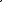
\includegraphics[width=.3\textwidth]{4x4}
\caption{inputLayerSize = 4; middleLayerSize = 1; numberOfSpecies = 50; maxIteration = 1000; maxError = 0.000017; mutationRatio = 0.6; crossoverRatio = 0.1}
\end{figure}
Wynik okazał się identycznyz obrazem wejściowym. Program zakończył swoje dzialania po kilkunastu iteracjach, gdy błąd przekroczył granicę maxError.

Następnie przetestowaliśmy poniższy obraz:

\begin{figure}[h]
\centering

\includegraphics[width=.3\textwidth]{gray2s}
\caption{Obraz wejściowy złożony z dwóch pasków: czarnego i białego o rozmiarze 8x8}
\end{figure}

\begin{figure}[H]
\centering
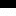
\includegraphics[width=.3\textwidth]{gray2s-o}
\caption{Obraz wyjściowy. Parametry: inputLayerSize = 64; middleLayerSize = 4; numberOfSpecies = 100; maxIteration = 5000; maxError = 0.00001; mutationRatio = 0.9; crossoverRatio = 0.1}
\end{figure}

Program zakończył się po kilku tysiącach iteracji przekraczając błąd. Mimo małego maxError widać delikatne artefakty. Następne testy przeprowadziliśmy z krótszymi wektorami wejściowymi. Jako obraz testowy wzięliśmy zębatkę:

\begin{figure}[H]
\centering

\includegraphics[width=.4\textwidth]{cog}
\caption{Obraz wejściowy}
\end{figure}

\begin{figure}[H]
\centering

\includegraphics[width=.4\textwidth]{cog4}
\caption{Obraz wyjściowy. Parametry: inputLayerSize = 4; middleLayerSize = 2; numberOfSpecies = 100; maxIteration = 500; maxError = 1; mutationRatio = 0.5; crossoverRatio = 0.1}
\end{figure}

\begin{figure}[H]
\centering

\includegraphics[width=.4\textwidth]{cog16}
\caption{Obraz wyjściowy. Parametry: inputLayerSize = 16; middleLayerSize = 2; numberOfSpecies = 100; maxIteration = 800; maxError = 1; mutationRatio = 0.9; crossoverRatio = 0.1}
\end{figure}

Dla obrazu z inputLayerSize=4 program się skończył, ponieważ błąd został przekroczony, natomiast dla drugiego przypadku (z 16 neuronami wejściowymi) po 800 iteracjach błąd wynosił 13.


\section{Podsumowanie}
Wyniki testów pokazują, że założony w dokumentacji wstępnej rozmiar wektora wejściowego (64) jest użyteczny tylko dlla prostych obrazków. Nawet testy z użyciem wektora o długości 16 dały umiarkowane wyniki. Widać z kolei, że testy, w których długość wektora wejściowego jest równa 4 dają dobre rezultaty - nawet dla skomplikowanych obrazów. Warto też zauważyć, że dla tych obrazow w warstwie pośredniej był tylko 1 neuron. Według naszych przewidywań sieć byłaby w stanie się nauczyć trudnych obrazów również dla sieci o większych rozmiarach, ale wymagałoby to dużego czasu uczenia.

\end{document}
